\section{ Dimensionality Reduction Methods}
In the last section we described a number of methods in which the chemical structure of a species could be incoded for direct comparison. However since each input is made up of a multitude of elements, it is still not a simple task determine the differences and similarity between all species in a mechanims. Dimensionality reduction is the process of reducing the number of random variables and only presentind a set of principal values, by mapping a high-dimensional space into a low-dimensional one, \citep{drrandom}. This allows us to flatten a multivariate input into the two dimension required for a simple scatter plot.

In this section we begin by explaining the data preperation required for dimensionality reduction (\autoref{sec:pref}) before desribing the different possible methods of reducing the dimensions of a dataset. 

% 
% Computational algorithms are often described as a black box. This is due to their structure, where we begin with a set of inputs, $X$. These then have a series of operations applied to them, $f(X)$, eventually producing the corresponding output $Y$. In the case of simple linear regression, this intermediate process may be calculated easily by hand. Unfortunately for large datasets, or complex iterative models, this becomes somewhat impractical. Additionally, algorithms such as neural networks or genetic (evolutionary) algorithms may also require the changing of items or hyper-parameters in-situ.
% It is for this reason models need to be evaluated, ensuring that they not only run correctly but register the correct set of features we are interested in.
% 
% For predictive models, an adaptation of the leave-one-out method of assessment is commonly applied. Data is split into a $2/3:1/3$ ratio, whereupon the model is trained on two-thirds of the data, and evaluated in its predictive capabilities on the remaining third. This process is repeated with many permutations of the data to determine an overall model variance. Unfortunately, since we wish to use machine learning (ML) for exploratory data analysis, we need to take a different approach to evaluating the usefulness of a model. Here we take a known property, which through prior knowledge should be highlighted by the models, and compare the output categories output with these.
% 
% 
% \begin{figure}[H]
%   \centering
%   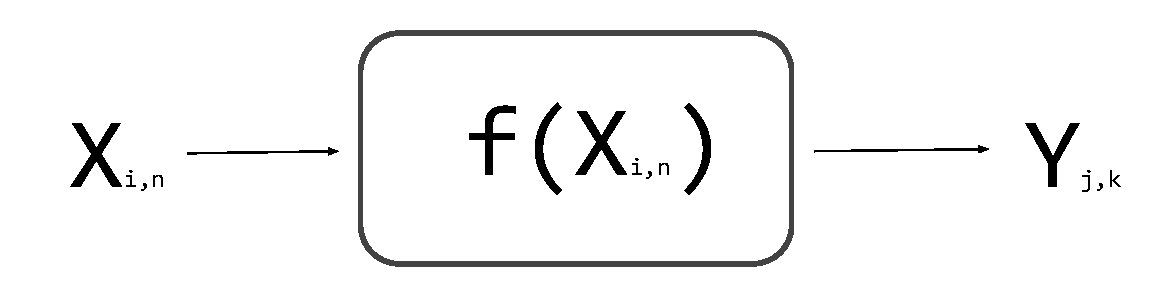
\includegraphics[width=.5\textwidth]{4fig/xy.pdf}
%   \caption{The general flow chart of flow within a machine learnt model.}
%   \label{xy}
% \end{figure}


\subsection{Preperation of the data}\label{sec:prep}
Real-world data is rarely preformatted in such a way that it can be used directly within a computational model. Often values need to be cleaned and corrected to be fit for purpose. In the interest of completeness the two main methods of data adjustment for machine learning are outlined below. These are normalisation and standardisation. 


\subsubsection*{Normalisation}
In the data is without (dimensionless) or of a single unit, it is poissble to rescale the data between a range - most commonly {0,1}. In doing so it is possible to interperate the importance of a value in contrast to the largest recorded value. This gives us a percentage scale spanning the range of the data. Such a range is useful in the definition of colourmaps and describing a values importance relative to the dataset. 
To rescale a dataset we shift the minimum value to zero, then divide by the new maximum of the dataset (Note this is equivalent to the range of the unshifted dataset.)

\begin{equation}
    n(x_i) = \frac{x_i - \min_x }{\max_x - \min_x}
    \label{eqn:n}
\end{equation}



\subsubsection*{Standardisation}
If the components we wish to compare are of differing units, or are expressed with a different scale, normalising them would not produce meaninful data. Instead it is possible to standardise the data by looking at each points deviation from the mean. This is done by dividing the variation of each point from the mean by the standard deviation of $S$ and results in a value between \{-1,1\}, \autoref{eqn:z}. In statistics this is known as the `z-score'\footnote{Possibly because of the American spelling of standardi\textbf{Z}ation?}

\begin{equation}
    z(x_i) = \frac{x_i - \mu_x}{S}
    \label{eqn:z}
\end{equation}\\    


\subsection{Principle Component Analysis}
One of the most well known dimensionality reduction methods is the determination of the principal components through the use of Principal Component Analysis (PCA). PCA works on the assumption that components within a dataset are linear combinations of eachother. By simplifying these linear combinations, it is possible to identify the components which explain the most variability in a dataset - these are the principal components \citep{pca,pca2}.

A simpler interpretation of this would be to adjust the direction of each axis of the data, such that its projection has the largest variability. In doing so it is possible to determine which components contribute the most to changes in the dataset. An example of this is seen in \autoref{fig:2dpca} where the second component of the original data may be removed with little effect on the overall result of the data. Such methods have applications in compression and signal filtering [REF REF]


\begin{figure}[h]
    \centering
    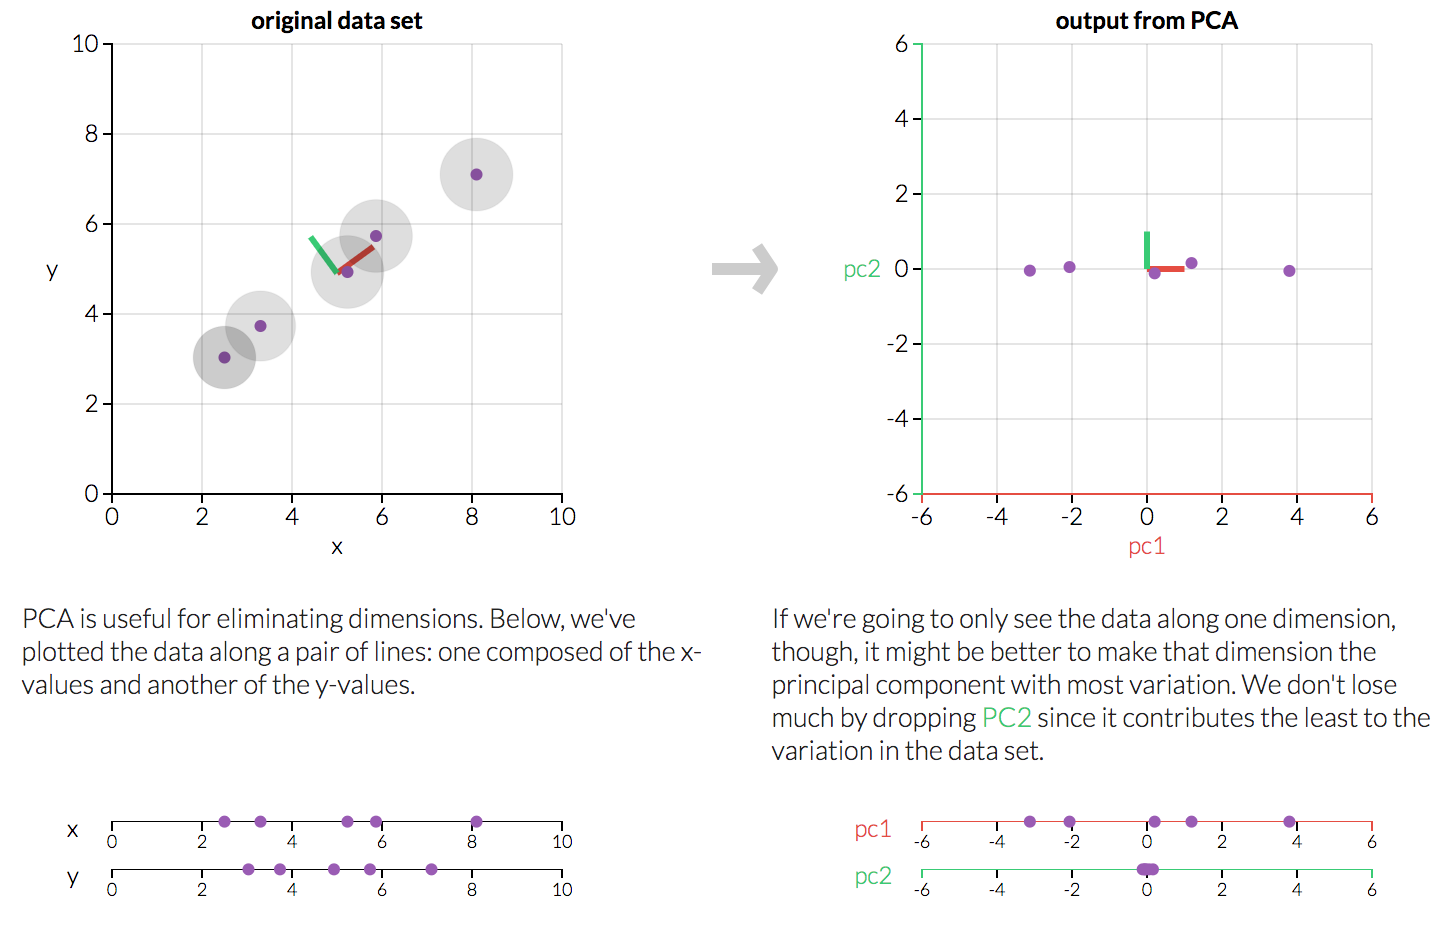
\includegraphics[width=.8\textwidth]{./4fig/pca2d.png}
    \caption{\textbf{Determining the Principal Compnent of a sample dataset.} It can be seen that in a change in axis to follow the first principal component (right), it is possible to explain most of the variation in the samle dataset (left). Source: \citep{pcaim}}
    \label{fig:2dpca}
\end{figure}


\subsubsection{Mathematical explanation of PCA}
\emph{\textbf{Note:} The basic statistics/mathematics required to understand this section is shown in \autoref{apendix:pca}. Please read this if you are not familiar with any of the terms below.
}

The mathematics behind PCA consists of first calculating the covariance matrix. This is an $n \times n$ matrix outlining how strongly each variable changes with every other. Using this we can calculate both the eigenvalues and eigenvectors of the matrix \footnote{These need to be unit vectors, although most packages already do this out of the box.}. This may be done using a computational package such as numpy or scipy \citep{numpy,scipy}.

We can now sort the eigenvector columns by influence using their eigenvalues. This way a feature data-set can be produced by removing vectors of low influence. The final feature dataset can now be transposed and multiplied by the transpose of the original dataset. This produces an output dataset containing each principal component of the desired dimension.



\subsection{t-Distributed Stochastic Neighbor Embedding (t-SNE)}

t-SNE is an algorithm designed with visualisation in mind \citep{tsne}. Rather than representing the data through a series of linear transformations, t-SNE uses local relationships to create a low-dimensional mapping, much in the same way as a fully connected force graph, \autoref{fig:tsneforcegraph}. This allows the ability to capture non-linear structures in the data which cannot be done through linear mapping methods (e.g. PCA).

The algorithm itself can be broken down into two parts[REF ttsne introduction paper]:
\begin{itemize}
  \item [1.] Create a probability distribution which dictates relationships between neighbouring points
  \item [2.] Recreate a lower-dimensional space following the probability distribution established in 1.
\end{itemize}

The main reason t-SNE produces good results is that it can handle the `crowding problem' very well.


\subparagraph{Crowding Problem}\label{sec:overcrowd}
The crowding problem is a product of the `curse of dimensionality. This is because, in high dimensional space, the surface of a sphere will grow much quicker than one in a lower dimension space. This means higher dimension spaces will have more points at a medium distance from a certain point, \autoref{fig:dimcurse}. When we map our data into a lower dimension, data will try to gather at its medium distance, resulting in a more `squashed', and thus crowded, output.



\begin{figure}[H]
  \centering
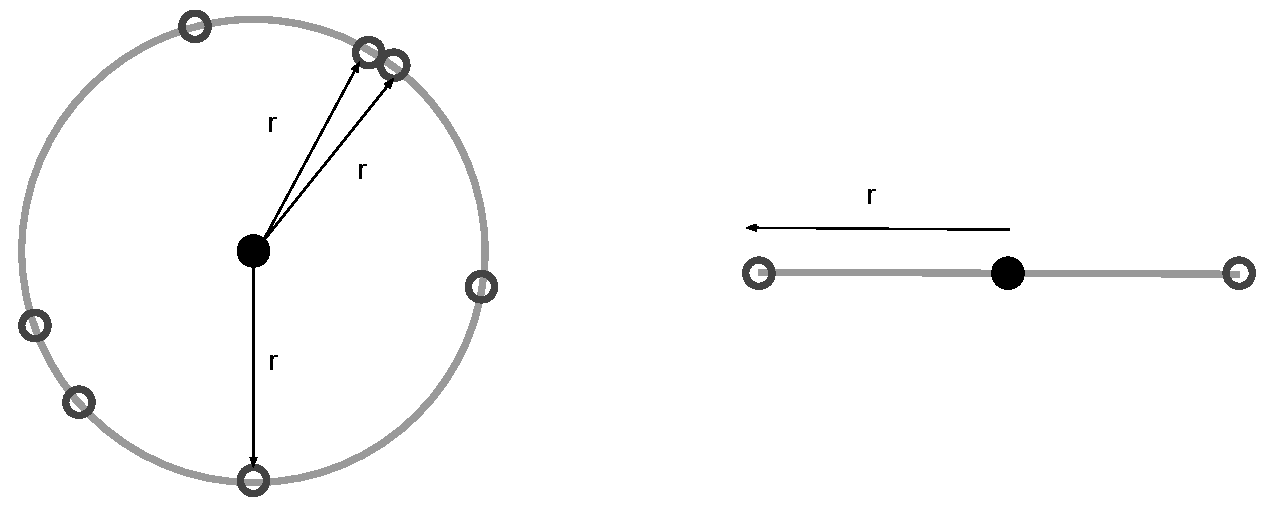
\includegraphics[width=.5\textwidth]{4fig/dimcurse.pdf}
\caption{An example of how the curse of dimensionality affects the mapping of points a certian distance from eachother. }\label{fig:dimcurse}
\end{figure}




\subsubsection{Mathematical explanation of t-SNE}
%https://mlexplained.com/2018/09/14/paper-dissected-visualizing-data-using-t-sne-explained/

%
% The general process is given by the etymological dissection of the acronym, with `t'  standing for the student T probability distribution and S, N (stochastic and neighbour) explaining the use of the distribution across neighbouring points in space.

In the original paper \citep{tsne}, the algorithm is described using the etymologic dissection of its name.

\paragraph{Step 1}
First we begin with Stochastic Neigbour Embedding (SNE) - the distribution across neignbouring datapoints in our high dimension space. This is done by converting the high dimensional Euclidian distances between points into conditional probabilities representing their similarity:

\begin{equation}
p_{ij} = \frac{\exp(-\left \| x_i - x_j \right \|^2 / 2\sigma_i^2)}{\sum_{k \neq l} \exp(- \left \| x_k - x_l \right \|^2 / 2\sigma_i^2)}
\end{equation}

Here $p_{i|j}$ is the conditional probability that $x_i$ may pick $x_j$ as a neigbour. This is proportional to the probability density of a Gaussian $\sigma_i$ centered at $x_i$.

\subparagraph{Perplexity}
Since we want the number of neighbours of each point to be similar in number and prevent a single point from having a disproportionate influence on the entire system we introduce a hyperparameter named \emph{perplexity}. This works by ensuring that $\sigma_i$ is small for points in densely populated areas and large for spare ones. This means that the perplexity of a system can be thought of as a scale of the number of neighbours considered for any one point. Generally, values between 5 and 50 are considered to give good results, with larger perplexities taking global features into account, and by consequence smaller ones, local features.

\paragraph{Step 2}
Now a probability distribution describing the relationship between points has been formulated, we wish to express this as a low dimensional mapping of our inputs $X$ in terms of our output dimensions $Y$. Naturally, we would want to make the low dimensional mapping represent a similar (Gaussian) distribution as in Step 1. However, it often causes issues presented by the `overcrowding problem'\autoref{sec:overcrowd}. This is because the gaussian has a `short tail', and thus nearby points are likely to be pushed together. A solution to this is the student t-distribution which has a longer tail \footnote{The distribution employed is a t-distribution with only one degree of freedom. This is identical to the Cauchy distribution}:

\begin{equation}
q_{i|j} =\frac{(1 + \left \| y_i - y_j \right \|^2 )^{-1}}{\sum_{k \neq l} (1 + \left \| y_k - y_l \right \|^2 )^{-1} }
\end{equation}

\emph{\textbf{Note:} The definition and explination of the Student t-distribution is given in \autoref{apendix:tsne}.
}

The optimisation of this equation can be achieved through the use of \emph{gradient decent}\footnote{\textbf{Gradient Decent}
This is an optimisation algorithm used to minimise a function by iteratively moving in the direction of the steepest descent. This can be used to find local minima and is defined by the negative of the gradient. Its primary usage in machine learning is the updating of parameters (coefficients in linear regression and weight in neural networks).}
 on the Kullback-Leibler divergence \autoref{appendix:kl} between distributions $p$ and $q$. Here the gradient is used to apply an attractive and repulsive force on the items\footnote{A positive gradient signifies attraction, whilst a negative one corresponds to repulsion.}.




\subsection{PCA vs t-SNE, a quick comparison.}

PCA is one of the most used DR algorithms[ ref list ]. It is fast, simple and easy to use and very intuitive. The PCA algorithm works by creating a lower-dimensional embedding which best preserves the overall variance of the dataset. Clusters created from the algorithm are grouped in ways, such that they preserve the greatest variance.

The main drawback of PCA is that it is a linear projection. If our data happened to be in a `swiss roll' (spiral) pattern, we would not be able to `unroll' it. This is because PCA works by viewing the data from different perspectives, much like casting a shadow from various directions. With such an example, there is no one way we can do this that unfurls the spiral.

t-SNE, on the other hand, is a relatively new method [ref 06/08 paper]. Its greatest asset is that it is not limited by linear projections. Although more computationally intensive for large datasets, t-SNE produces visibly cleaner results. Unlike in PCA, t-SNE cannot be trained on additional data at a later point, however, the output clusters are more visually distinct (they have less overlap). Much like in a force graph, the output from t-SNE is scale-invariant. This means that whilst the location of clusters in a PCA reduced representation have an attributable quality, those produced by t-SNE will not necessarily contain the same information.

To test the differences between the two methods, a box model run representative of the chemistry within Beijing was used. The aim was to classify the diurnal profiles of each species concentration. To do this we standardised all the results and extracted the third day from a spun up model. These results were then fed into both the PCA and t-SNE algorithm. \autoref{fig:threegraphs} show the differences between the models. In \autoref{fig:pcac} we can see that the embedding is prone to overlap between species, with sample groupings (non-yellow species)\footnote{Species with similar profiles were grouped,\autoref{fig:tco} } often being densely stacked on top of each other and indistinguishable from collections of species around them. Although only a slight improvement for the specified dataset, the t-SNE reduction allows the points to be better distributed, improving the definition of the group boundaries.

\begin{figure}[H]
     \centering
     \begin{subfigure}[b]{0.495\textwidth}
         \centering
         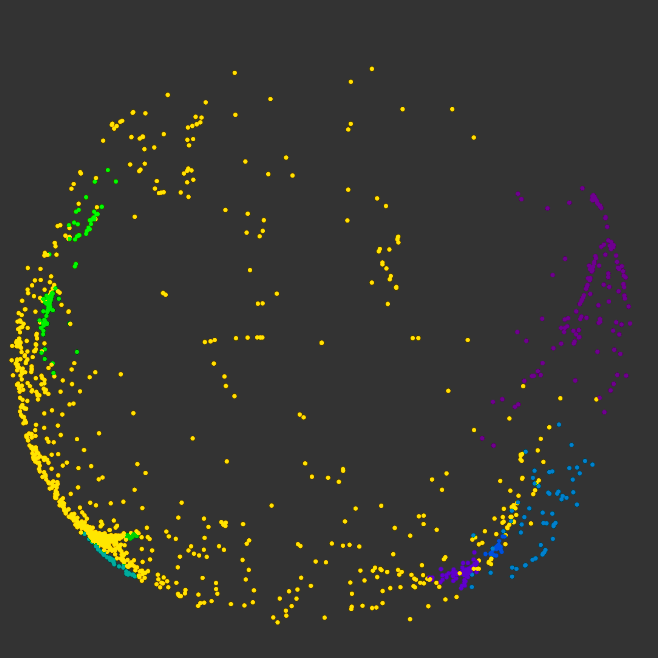
\includegraphics[width=\textwidth]{4fig/ppca.png}
         \caption{PCA}
         \label{fig:pcac}
     \end{subfigure}
     \hfill
     \begin{subfigure}[b]{0.495\textwidth}
         \centering
         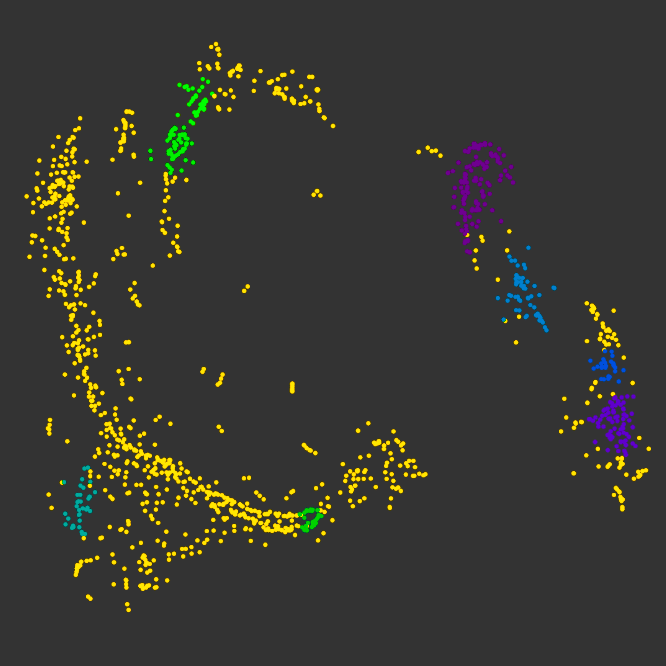
\includegraphics[width=\textwidth]{4fig/ptsne.png}
         \caption{t-SNE}
         \label{fig:tsnec}
     \end{subfigure}
     \hfill \hfill
     \begin{subfigure}[b]{\textwidth}
         \centering
         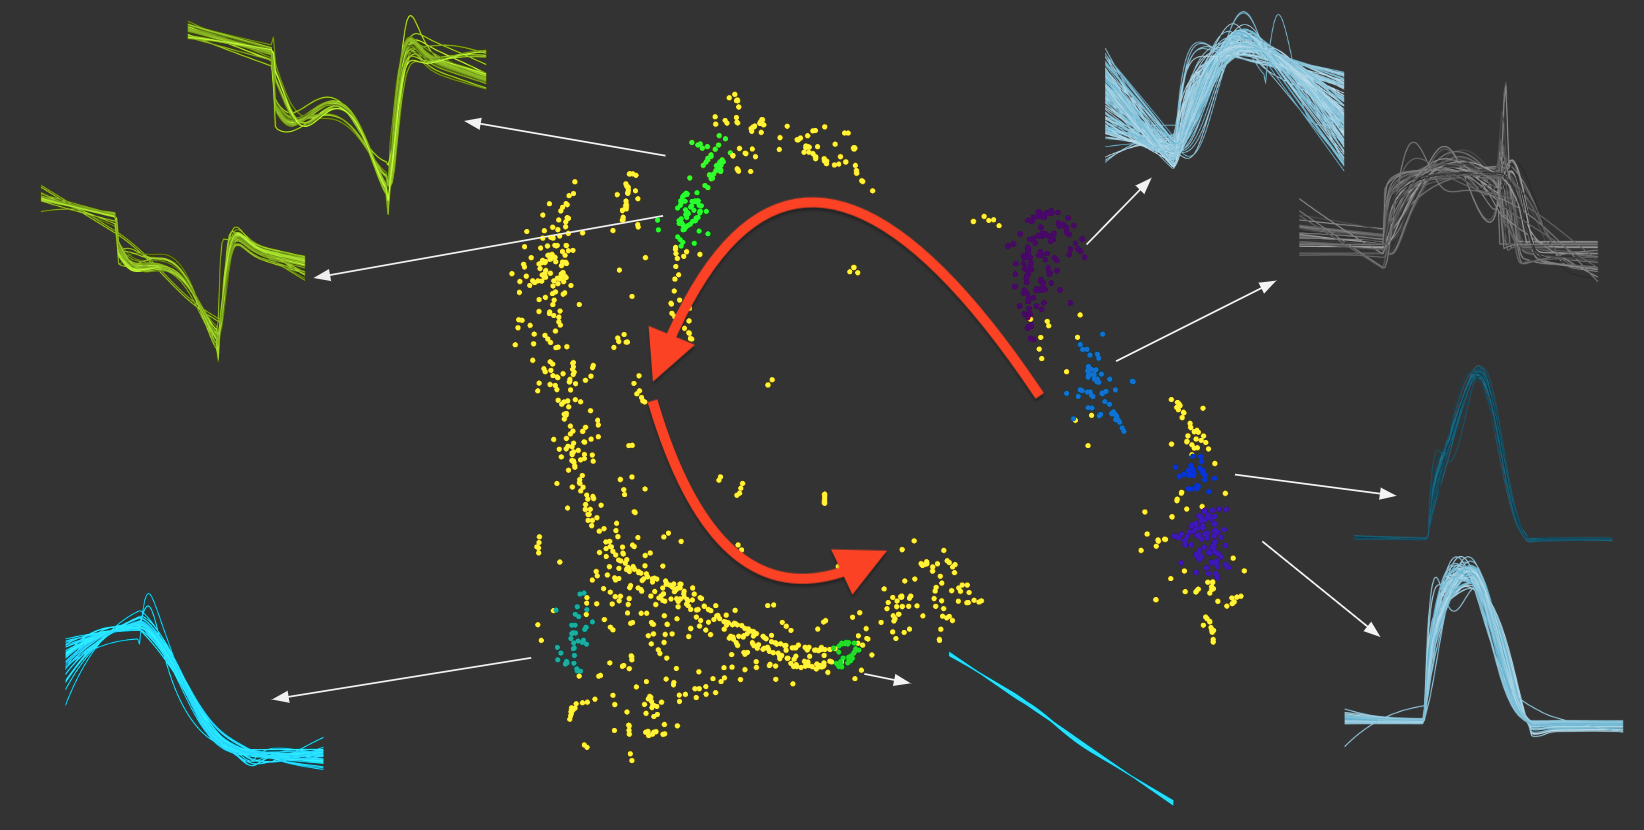
\includegraphics[width=\textwidth]{4fig/ptsneall.png}
         \caption{t-SNE with cluster outlines.}
         \label{fig:tco}
     \end{subfigure}
        \caption{Three simple graphs}
        \label{fig:threegraphs}
\end{figure}




\subsection{The Auto-Encoder (AE)}
Auto-encoders are a subclass of neural networks which are primarily used for dimensionality reduction. Rather than predicting a numerical output autoencoders focus on the construction and deconstruction of data through the use of an encoder and decoder pair. The encoder takes an n-dimensional input and applies a compression, reducing it to the number of dimensions in the bottleneck layer. This reduced dataset is then reconstructed within the decoder. Such a process not only allows for an easy understanding of the error of the reduced data but can also be used in the filtration of noisy or pixelated data [ref].\\


\begin{figure}[H]
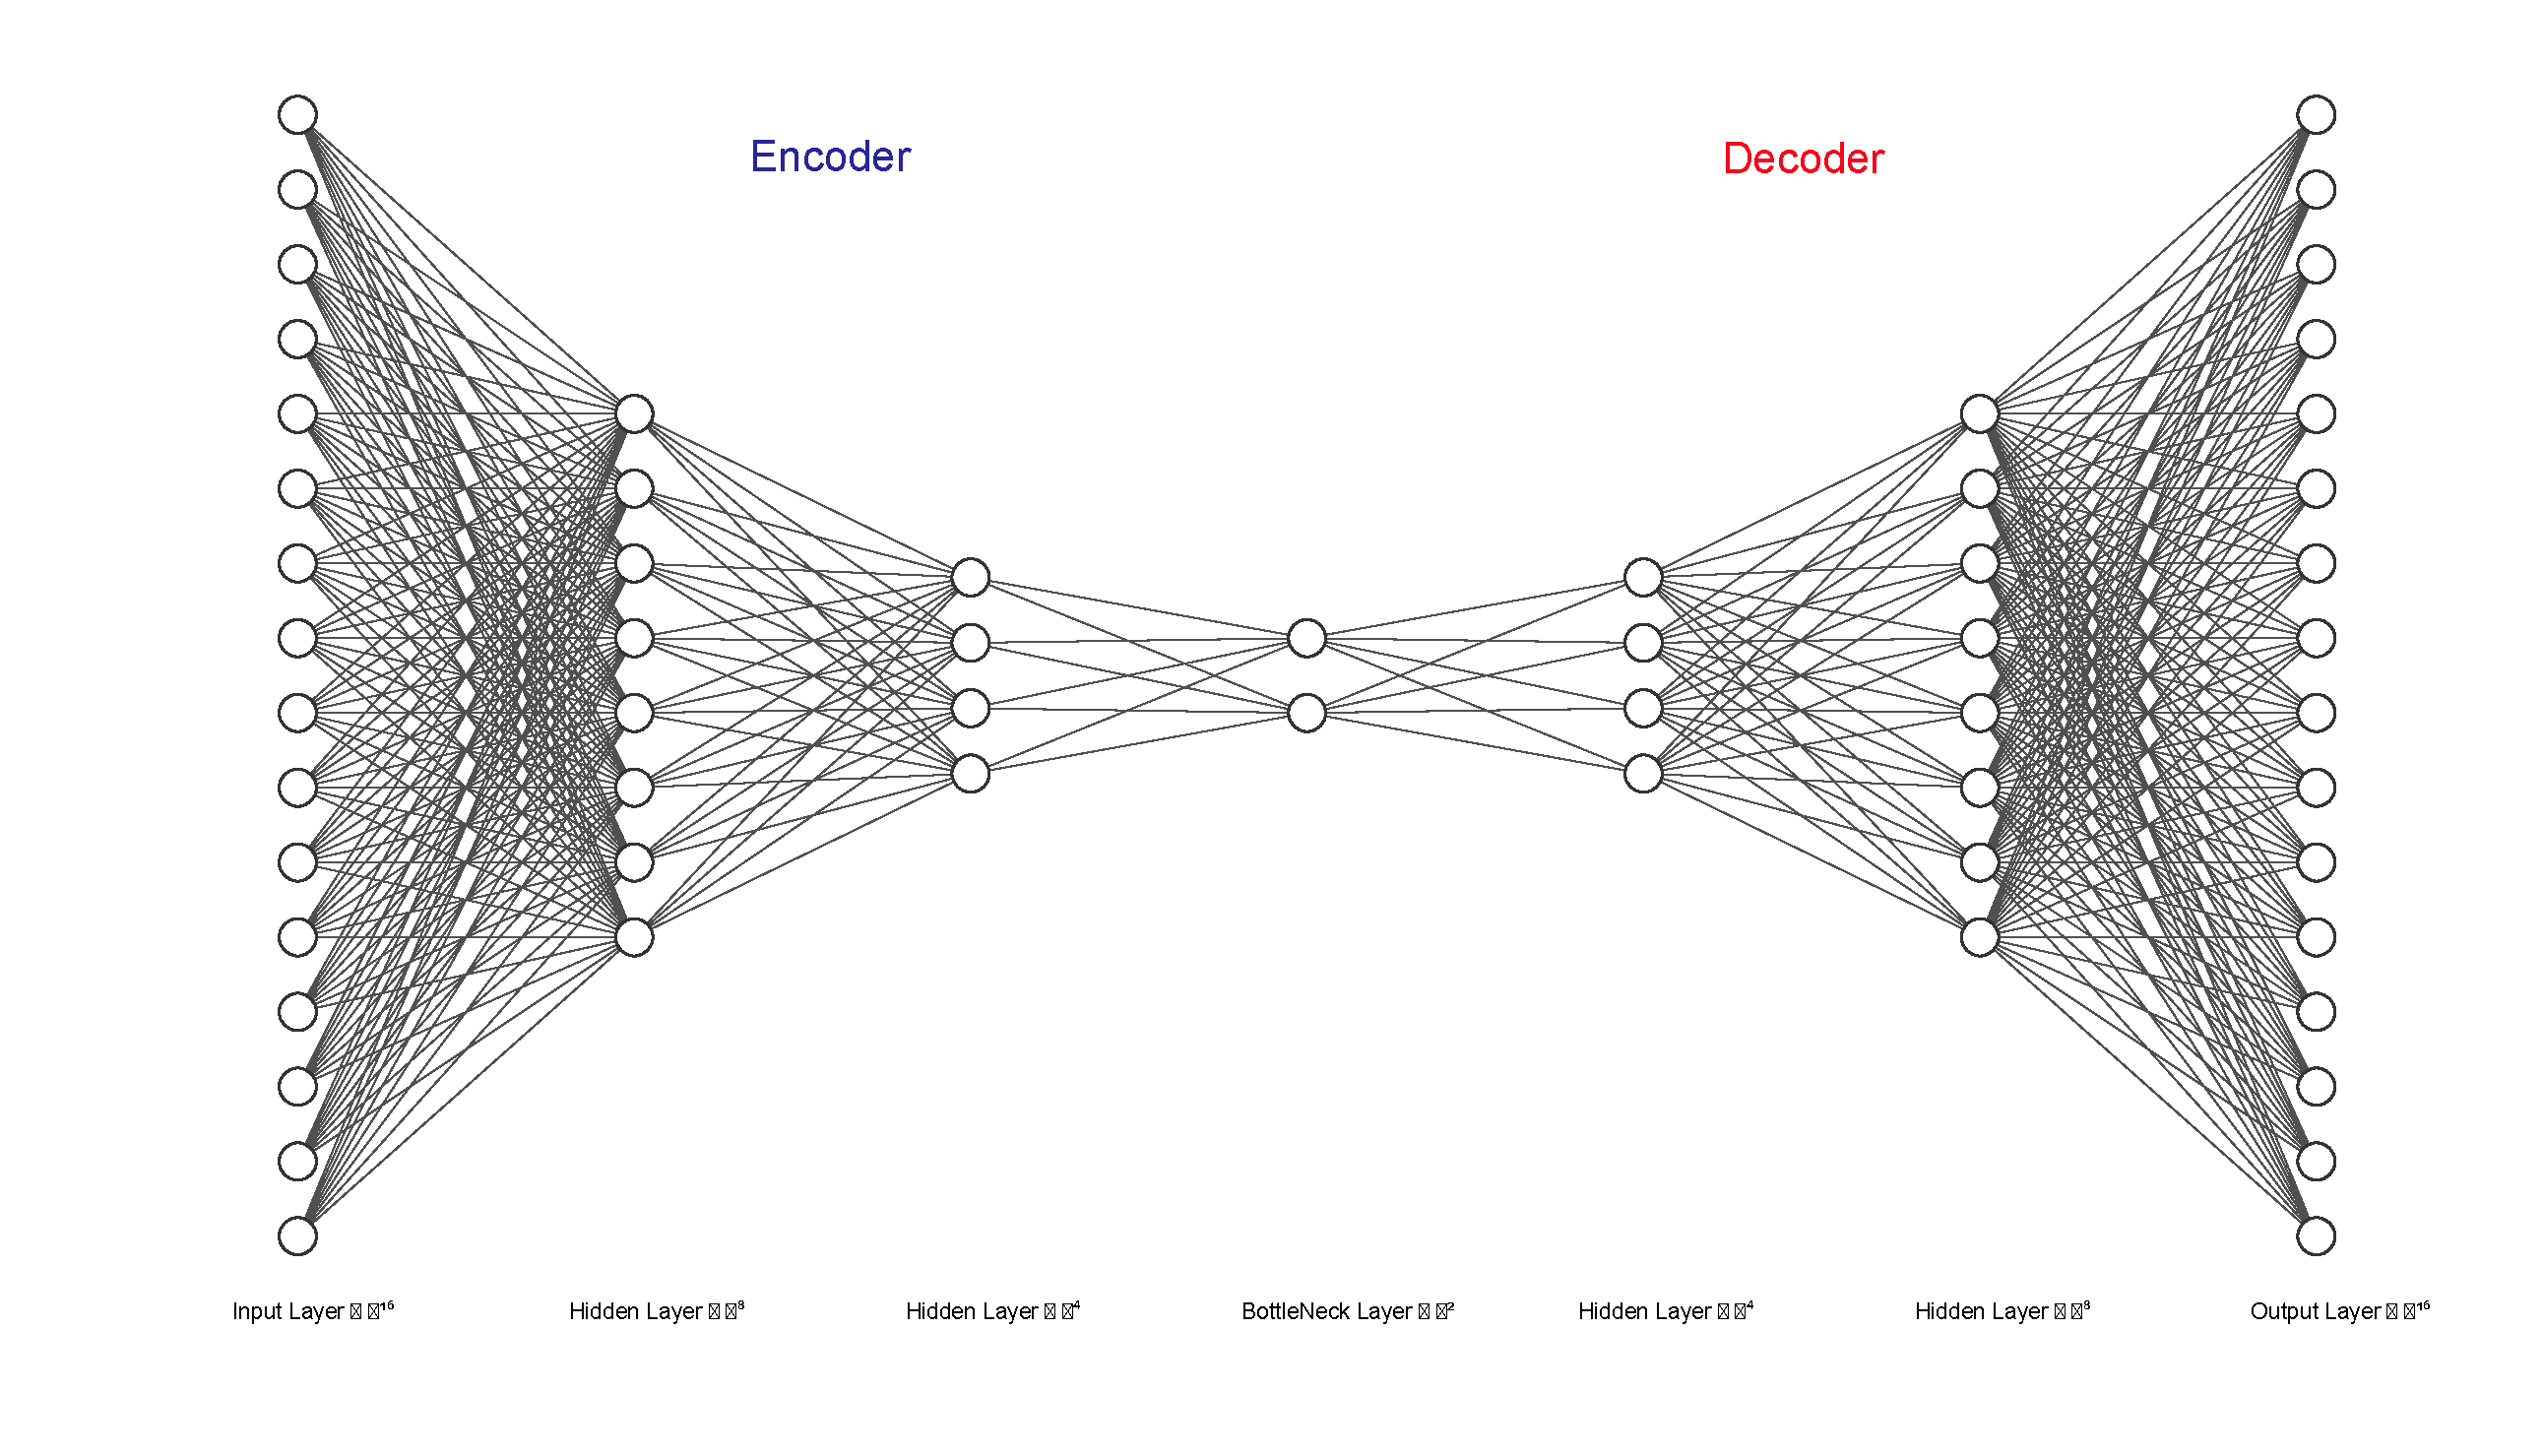
\includegraphics[width=\textwidth]{4fig/ae.pdf}
\caption{An example autoencoder structure which reduces a 16 dimentional input to 2. Draw with the aid of \citep{drawae}}
\end{figure}


Usage in image reconstruction, signal processing or feeding large data into other models. \\

There are two features of an autoencoder that make it powerful. The first is the ability to sample your latent space using the decoder. This means we can establish features that correspond to gaps between our data points - which can have its application if the data used is sparse or incomplete. Next comes the inherent non-linearity of the model. As an autoencoder is just a neural network, the amount of information passed through each link between layers is governed by an activation function. Should this activation function be linear, the reduced dimension will be much akin to a PCA decomposition. However unlike PCA, in reducing the number of dimensions, we do not discard any data, but rather combine it - as per the nature of the links of the network. In trying to model/fit non-linearity, we have a range of activation functions to choose from. These are:



\subsubsection{Demonstration of non-linear activation functions}

To demonstrate the effect of these we take a sample isopleth of Methane and Ozone, reduce it to two dimensions, and then reconstruct it. Here we can see that some of the non-linearity of the original dataset has been lost when discarding the third principal component during PCA. Using a tanh activation function in an auto-encoder however, recreates much of the original properties of the data.


\begin{figure}[H]

\begin{subfigure}{.33\textwidth}
  \centering
  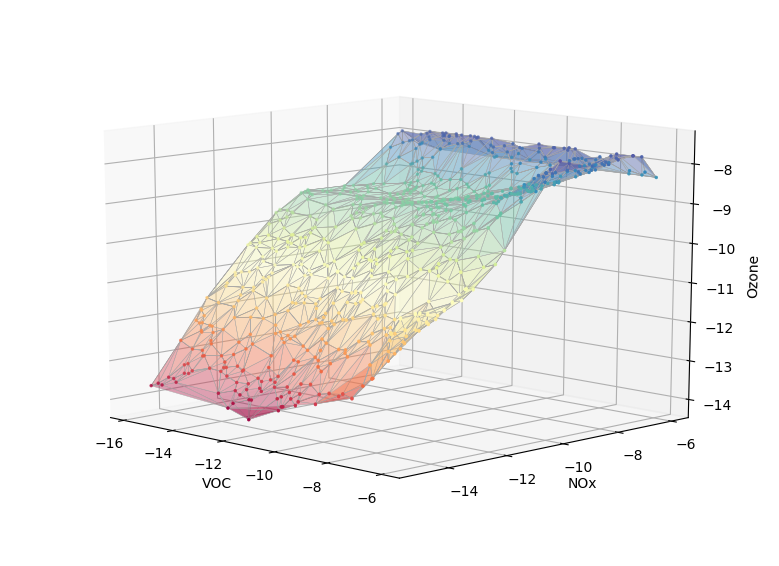
\includegraphics[width=\textwidth]{4fig/original.png}
  \label{fig:orig}
  \caption{Original}
\end{subfigure}%
\begin{subfigure}{.33\textwidth}
  \centering
  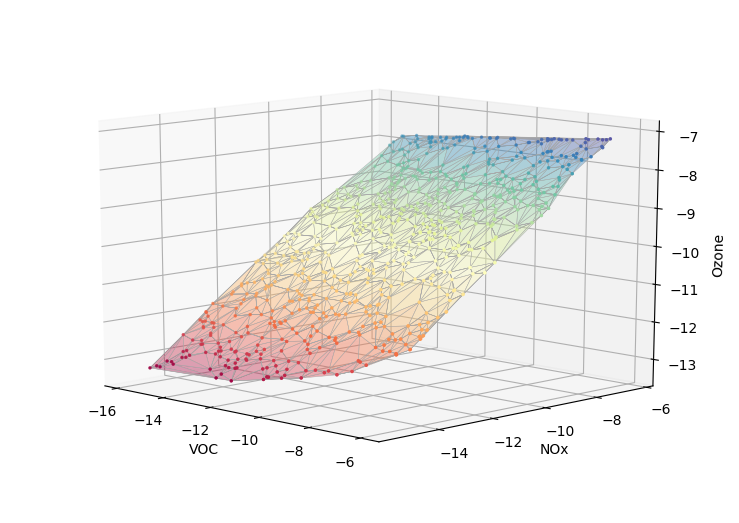
\includegraphics[width=\textwidth]{4fig/rpca.png}
  \label{fig:pca}
  \caption{PCA}
\end{subfigure}%
\begin{subfigure}{.33\textwidth}
  \centering
  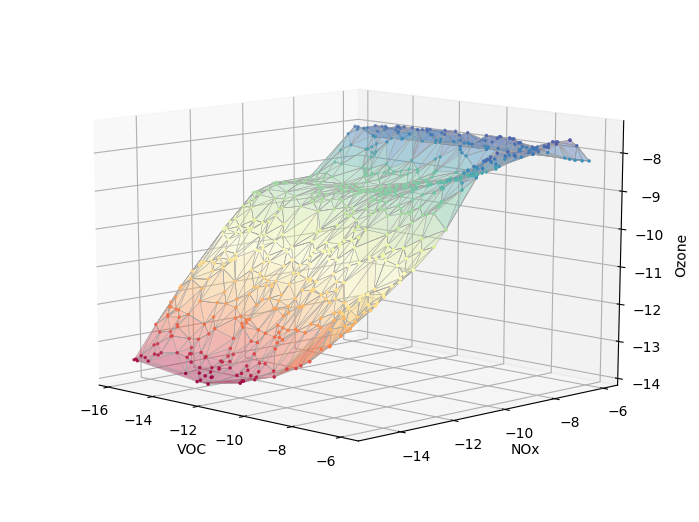
\includegraphics[width=\textwidth]{4fig/rae.png}
  \label{fig:ae}
  \caption{AE (Tanh)}
\end{subfigure}%


\caption{Reducing the original dataset by 1 dimension and reconstructing it using different methods. Figure created using 300 simulations initialised with NOx (variable), Methane (variable) and Ozone (constant) using a Latin hypercube. The results are then plotted and converted into a surface using Delaunay triangulation. }
\end{figure}

%
% \subsection{Graph Auto-Encoders (GAE)}
%
% It was seen that graphs neural networks (GNN) were far more powerful in 2016...
% Training time and results\\
%
% Graph auto-encoders are an extension to these, applying the auto-encoder structure to a GNN. Here we may feed information about the relationships between items in our network, as well as the features representing them.
%
% This method of representation has its purpose in both classification and link prediction. In terms of an autoencoder, we may use this to extract the graph embeddings at a lower dimension. In \citep{karatAE} it is shown that GAEs are able to extract an embedding of the graph communities within a network. In other papers, GAEs have been used for matrix completion, and in-turn link prediction \citep{gaelink}. This makes them a potentially powerful tool in the visualisation, understanding and prediction of atmospheric chemical graphs.


\subsection{Node2Vec}\label{sec:n2v}
 Node2Vec is an embedding algorithm designed to generate vector representations of the nodes in an \textit{undirected} and \textit{unweighted} network. This not only allows the input of graph derived relationships into other models, but can also be more computationally efficient, by circumventing the need for expensive composition, whilst producing better predictions on some network-related tasks compared to more classical methods, such as PCA \citep{node2vec}.


\begin{figure}[H]
  \centering
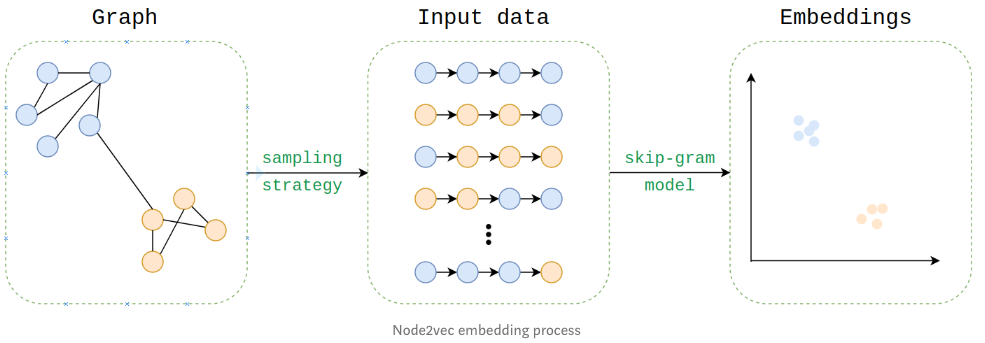
\includegraphics[width=\textwidth]{4fig/n2vproc.png}
\caption{The process of converting a graph into a vector using Node2Vec. Source:\citep{n2vimg}}\label{fig:n2vprocess}
\end{figure}


The process of converting the graph structure (\autoref{fig:n2vprocess}) into a numerical vector node embedding starts by taking a series of $2^{nd}$ order random walks. These describe the neighbourhood of a node in the form of a set of random walk paths, much in the same way words are dependant on their neighbours within a sentence: \autoref{eqn:w2varrow}.


\begin{equation}
ISOPRENE \rightarrow OH \rightarrow TISOPA \rightarrow ISOPBO_2 \rightarrow TISOPA \rightarrow...
\label{eqn:w2varrow}
\end{equation}


\subsubsection{Input / Sampling}
The probability and path depend both on a set of arguments and a random seed provided to the model. The return and input parameters $p,q$ determine how fast we explore the network and our probability to leave the neighbourhood, \autoref{fig:n2vedge}. In a network, where the previous path is from $t$ to $v$, we may calculate the probability of returning to $t$ as $1/p$, going to a mutual node connected between $t$ and $v$ as 1, and viewing a new node as $1/q$.
If $q>1$ we have a high probability to end up at nodes close to $t$, and with $q<1$ we are likely to explore other nodes. Additionally if we chose $p> \max{q,1}$ we are less likely to return to an already visited node ($p < \min{q,1}$ is likely to generate a backwards step). Since we wish to generate a `local' view, but do not wish to return to $t$ we select  $q \ge 1$ and $p > q$ our parameters as  $p = 2.0,q=1.1$.  In the case of a weighted graph (something that we are \textit{not} exploring within this chapter) the resultant $alpha$ value calculated is further multiplied by the edge weight.

To run the simulation we use the python 2 code provided by the original paper \citep{node2vec} with a set of 50000 random walks, each of length 9. The reasoning behind this is that we have a large graph, with a power-law like structure (within only a couple of steps we are connected to every other species within the network - that is if we do not include the inorganics, which in this case we are).

\textit{NOTE: This process takes over a week to compute, and then the binary file containing all walks in character form approaches 10 GB, for the complete MCM. ...in serial... }

\begin{figure}[H]
  \centering
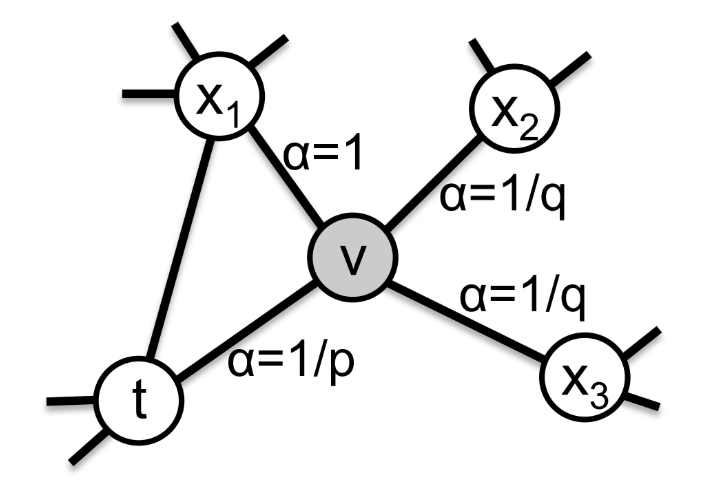
\includegraphics[width=0.5\textwidth]{4fig/n2vedge.png}
\caption{Calculation of the random walk path. Source:\citep{node2vec}}\label{fig:n2vedge}
\end{figure}

\subsubsection{Word2Vec}
Once we have constructed our random path `sentences', we can make use of the well renowned word2vec algorithm developed by Google \citep{w2v}. The word2vec algorithm is similar to an auto-encoder in many regards, but rather than learning word embeddings through reconstruction, it looks at the words (or species in our case) which neighbour each other in our corpus. This form of representation has found many uses beyond the realm of natural language processing. Some of these are objects, people, code, tiles,genes and graphs \citep{objects,people,code,tile,gene,graph2vec}.



https://skymind.ai/wiki/word2vec
http://mccormickml.com/2016/04/19/word2vec-tutorial-the-skip-gram-model/
